\documentclass[12pt]{article}
\usepackage{pgfplots}
\pgfplotsset{compat=1.17}

\begin{document}

\begin{figure}[h]
    \centering
    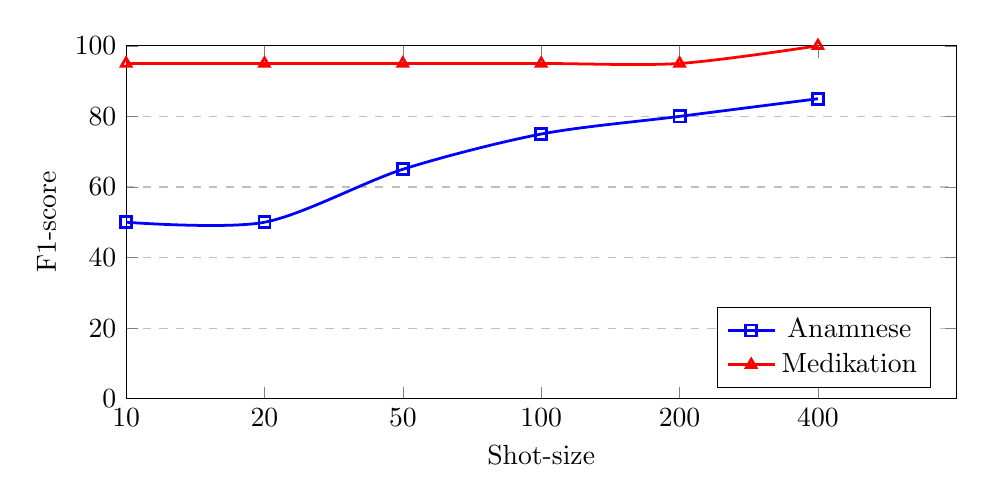
\begin{tikzpicture}
        \begin{axis}[
            title={},
            xlabel={Shot-size},
            ylabel={F1-score},
            xmin=0, xmax=6,
            ymin=0, ymax=100,
            xtick={0,1,2,3,4,5},
            xticklabels={10, 20, 50, 100, 200, 400},
            ytick={0,20,40,60,80,100},
            legend pos=south east,
            ymajorgrids=true,
            grid style=dashed,
            width=\linewidth,
            height=0.5\linewidth
        ]
        
        % Anamnese data (blue squares)
        \addplot[
            color=blue,
            mark=square,
            mark options={solid},
            line width=1pt,
            smooth,
            tension=0.5
        ] coordinates {
            (0,50)   (1,50)   (2,65)   (3,75)   (4,80)   (5,85)
        };
        
        % Medikation data (red triangles)
        \addplot[
            color=red,
            mark=triangle,
            mark options={solid},
            line width=1pt,
            smooth,
            tension=0.5
        ] coordinates {
            (0,95)   (1,95)   (2,95)   (3,95)   (4,95)   (5,100)
        };
        
        \legend{Anamnese, Medikation}
    \end{axis}
    \end{tikzpicture}
    \caption{\textbf{Core experiments: Primary class F1-score for all shot sizes}. F1-score per few-shot sizes for primary classes with no context using \textit{gbert-base-comb nocontext}.}
\end{figure}

\end{document}